% \iffalse
\let\negmedspace\undefined
\let\negthickspace\undefined
\documentclass[journal,12pt,twocolumn]{IEEEtran}
\usepackage{cite}
\usepackage{amsmath,amssymb,amsfonts,amsthm}
\usepackage{algorithmic}
\usepackage{graphicx}
\usepackage{textcomp}
\usepackage{xcolor}
\usepackage{txfonts}
\usepackage{listings}
\usepackage{enumitem}
\usepackage{mathtools}
\usepackage{gensymb}
\usepackage{comment}
\usepackage[breaklinks=true]{hyperref}
\usepackage{tkz-euclide} 
\usepackage{listings}
\usepackage{gvv}
\def\inputGnumericTable{}                                 
\usepackage[latin1]{inputenc}                                
\usepackage{color}                                            
\usepackage{array}                                            
\usepackage{longtable}                                       
\usepackage{calc}                                             
\usepackage{multirow}                                         
\usepackage{hhline}                                           
\usepackage{ifthen}                                           
\usepackage{lscape}

\newtheorem{theorem}{Theorem}[section]
\newtheorem{problem}{Problem}
\newtheorem{proposition}{Proposition}[section]
\newtheorem{lemma}{Lemma}[section]
\newtheorem{corollary}[theorem]{Corollary}
\newtheorem{example}{Example}[section]
\newtheorem{definition}[problem]{Definition}
\newcommand{\BEQA}{\begin{eqnarray}}
\newcommand{\EEQA}{\end{eqnarray}}
\newcommand{\define}{\stackrel{\triangle}{=}}
\theoremstyle{remark}
\newtheorem{rem}{Remark}

\begin{document}

\bibliographystyle{IEEEtran}
\vspace{3cm}

\title{GATE EE23 27}
\author{EE23BTECH11043 - BHUVANESH SUNIL NEHETE$^{*}$% <-this % stops a space
}
\maketitle
\newpage
\bigskip

\renewcommand{\thefigure}{\theenumi}
\renewcommand{\thetable}{\theenumi}

\bibliographystyle{IEEEtran}

\textbf{Question:}
Which of the following statement(s) is/are true?
\begin{enumerate}[label=\alph*)]
    \item If an LTI system is causal, it is stable.
    \item A discrete time LTI system is causal if and only if its response to a step input $u\sbrak{n}$ is 0 for $n<0$.
    \item If a discrete time LTI system has an impulse response $h[n]$ of finite duration the system is stable.
    \item If the impulse response $0<|h\sbrak{n}|<1$ for all $n$, then the LTI system is stable.
\end{enumerate}
\solution
\begin{enumerate}
    \item
    \begin{align}
        \text{Assume}\quad h\brak{t}&=e^{2t}\cdot u\brak{t}\\
        \mathcal{L}\{e^{2t}\} &= \frac{1}{s-2}\quad Re\brak{s}>2
    \end{align}
    This system is causal but not stable because ROC does not contian imaginary axis.
    
    \begin{figure}[ht]
    \renewcommand\thefigure{1}
        \centering
        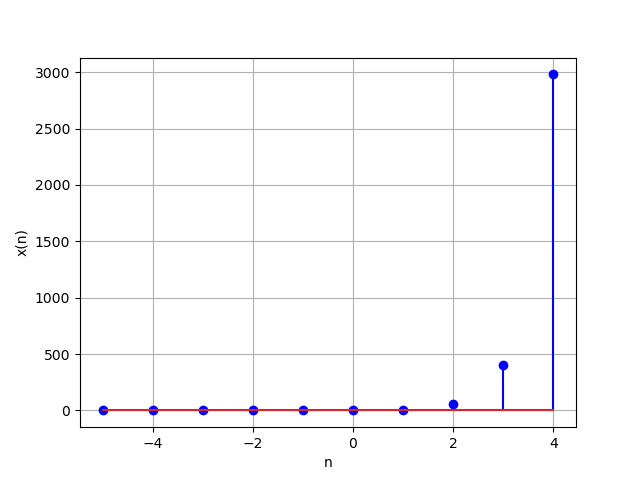
\includegraphics[width=0.8\linewidth]{figs/graph31.png}
        \caption{graph of $h\brak{t} = e^{2t}\cdot u\brak{t}$}
    \end{figure}
    Therefore, this statement does not hold true.
    \item
    \begin{align}
        \text{Assume}\quad h\sbrak{n} &= \begin{cases} 
                \frac{1}{3} & 0\leq n \leq 2 \\
                0 & \text{otherwise}
        \end{cases}\\
        y\sbrak{n}&=h\sbrak{n}*u\sbrak{n}\\
        y\sbrak{n}&=\sum_{k=-\infty}^{+\infty}h\sbrak{k}\cdot u\sbrak{n-k}\\
        &=\sum_{k=0}^{n}\brak{\frac{1}{3}}
    \end{align}
    Therefore, in this example, the system's response to a step input is indeed $0$ for $n<0$, fulfilling condition for causality.\\
    \begin{figure}[h!]
    \renewcommand\thefigure{2}
        \centering
        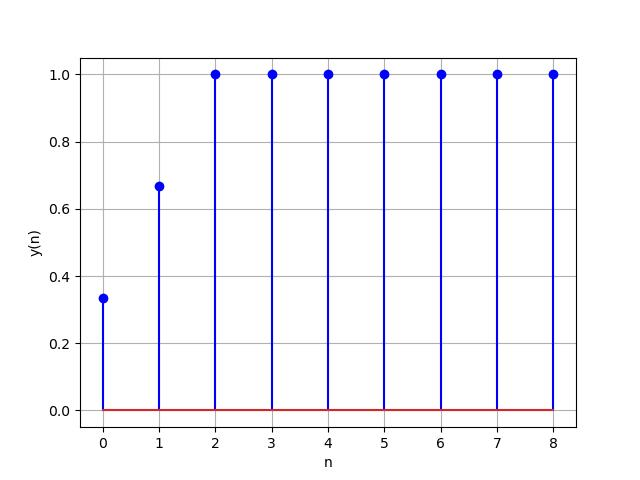
\includegraphics[width=0.8\linewidth]{figs/graph34.png}
        \caption{graph of $y\sbrak{n}$}
    \end{figure}
    Therefore, this statement is true.
    \item
    \begin{align}
            \text{Assume}\quad h\sbrak{n} &= \begin{cases} 
                n & \text{if}\hspace{2mm}0 \leq n\leq N\\
                0 & \text{otherwise} \\
        \end{cases}\\
        y\sbrak{n}&=h\sbrak{n}*u\sbrak{n}\\
        y\sbrak{n} &= \sum_{k=0}^nh\sbrak{k}u\sbrak{n-k}\\
        &=\sum_{k=0}^nk
    \end{align}
    The input response is finite but the output response in not BIBO stable.
    
    \begin{figure}[h!]
    \renewcommand\thefigure{3}
        \centering
        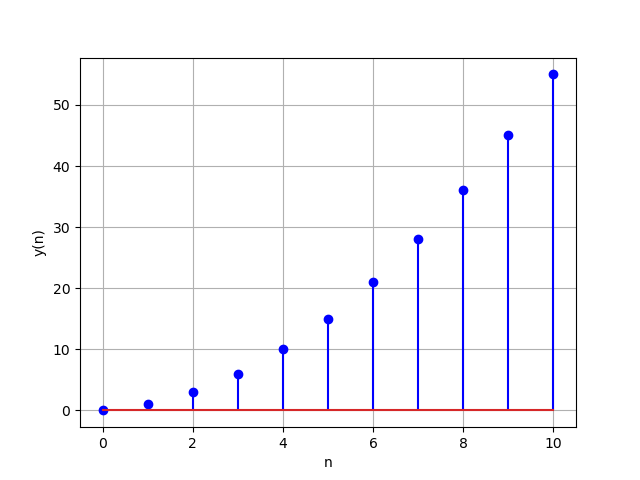
\includegraphics[width=0.8\linewidth]{figs/graph32.png}
        \caption{graph of $y\sbrak{n}$}
    \end{figure}
    Therefore, this statement does not hold true.
    \item
    \begin{align}
        \text{Assume}\quad h\sbrak{n}&=\frac{1}{2}u\sbrak{n}\\
        g\sbrak{n}&=\sum_{n=0}^{\infty}|h[n]|\\
        &=\sum_{n=0}^{\infty}\frac{1}{2}\\
        \implies\sum_{n=0}^{\infty}&|h[n]|\rightarrow \infty
    \end{align}
    Hence it is unstable.
    
    \begin{figure}[h!]
    \renewcommand\thefigure{4}
        \centering
        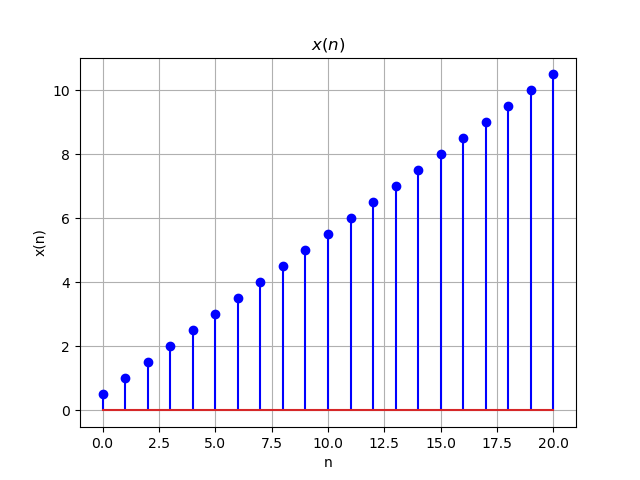
\includegraphics[width=0.8\linewidth]{figs/graph33.png}
        \caption{graph of $g\sbrak{n}$}
    \end{figure}
    Therefore, this statement does not hold true.
\end{enumerate}
So, the answer is option \brak{B}.

\end{document}
e
